\documentclass[czech,bachelor,dept460,male,csharp,cpdeclaration]{diploma}

\usepackage[autostyle=true,czech=quotes]{csquotes} % korektni sazba uvozovek, podpora pro balik biblatex
\usepackage[backend=biber, style=iso-numeric, alldates=iso]{biblatex} % bibliografie
\usepackage{dcolumn} % sloupce tabulky s ciselnymi hodnotami
\usepackage{subfig} % makra pro "podobrazky" a "podtabulky"

\usepackage{geometry}
\usepackage{listings}

\usepackage{mathtools}

\ThesisAuthor{Jan Jelička}

\ThesisSupervisor{Ing. Jan Janoušek}

\CzechThesisTitle{Webová služba pro sběr a vizualizaci předpovědí počasí}

\EnglishThesisTitle{Web service for collecting and visualizing weather forecasts}

\SubmissionYear{2021}

\Acknowledgement{Rád bych na tomto místě poděkoval vedoucímu bakalářské práce panu Ing. Janu Janouškovi, za pravidelné konzultace a poskytnutí mnoha užitečných rad a nápadů pro řežení samotné práce.}

% Zadame cestu a jmeno souboru ci nekolika souboru s digitalizovanou podobou zadani prace.
% Pokud toto makro zapoznamkujeme sazi se stranka s upozornenim.
%\ThesisAssignmentImagePath{Figures/Assignment}

% Zadame soubor s digitalizovanou podobou prohlaseni autora zaverecne prace.
% Pokud toto makro zapoznamkujeme sazi se cisty text prohlaseni.
%\AuthorDeclarationImageFile{Figures/AuthorDeclaration.jpg}


% Zadame soubor s digitalizovanou podobou souhlasu spolupracujici prav. nebo fyz. osoby.
% Pokud toto makro zapoznamkujeme sazi se cisty text souhlasu.
%\CooperatingPersonsDeclarationImageFile{Figures/CoopPersonDeclaration.jpg}

\CzechAbstract{Cílem bakalářské práce bylo vytvořit knihovnu, která bude schopna shromažďovat data o počasí z různých datových zdrojů v různých formátech (text XML, text JSON, bitmap). Agregovaná data jsou následně poskytována pomocí webové služby v jednom formátu (bitmap). Webová služba poskytuje data pro určité území v daném čase. Posledním bodem je vizualizační aplikace, která poskytuje uživateli možnost vykreslení počasí pro určité území v čase a také zobrazuje předpověď pro zadanou trasu.}

\CzechKeywords{XML; JSON; bitmap; počasí}

\EnglishAbstract{The aim of the bachelor thesis was to create a library that will be able to collect weather data from various data sources in various formats (XML text, JSON text, bitmap). The aggregated data is then provided using a web service in one format (bitmap). The web service provides data for a specific territory at a given time. The last point is a visualization application that provides the user with the ability to plot the weather for a certain area over time and also displays the forecast for the specified route.}

\EnglishKeywords{XML; JSON; bitmap; forecast}

\AddAcronym{XML}{Extensible Markup Language}
\AddAcronym{JSON}{JavaScript Object Notation}
\AddAcronym{BMP}{Bitmap}

\addbibresource{citace.bib}
\nocite{*}

% Zacatek dokumentu
\begin{document}
	
	\MakeTitlePages
	
	\chapter{Úvod}
	
	Informace o počasí jsou v dnešní době distribuována mnoha službami v různých podobách. Nejčastěji narážíme na textové formáty (XML/JSON) kde zprostředkovatelé dodávají kompletní výpis informací pro stát, město nebo konkrétní bod na základě zeměpisných souřadnic. Mimo textový formát narážíme i na snímky z radaru či barevné bitmapy, které poskytují předpověď pro rozsáhlou plochu v konkrétním čase. Předpovědi jsou vytvářeny pro různé časové intervaly na rozdílnou dobu dopředu, můžete tedy například narazit na předpověď obsahující data na 24 hodin dopředu s hodinovými rozestupy nebo na týden s vzájemnými rozestupy šesti hodin. Vzhledem k tomu že ke změnám počasí dochází relativně pomalu tak není potřeba znát data pro každou sekundu či minutu, stačí nám předpověď jednou za pár desítek minut případně i pár hodin.
	
	Cílem této práce je tedy sjednotit různé datové zdroje do jednotného formátu a vytvořit předpověď počasí pro určitou plochu v čase dle průměru těchto dat. Mimo to že každá služba může mít data ve svém formátu, je potřeba i sjednotit časy a především pozice pro které se data zjišťují.
	
	Dalším úkolem je vytvořit službu která bude schopna tyto agregovaná data poskytovat na základě dotazů uživatele. Uživatel může žádat o poskytnutí dat pro určitou plochu v patřičném čase, čímž obdrží patřičnou bitmapu. Případně může zažádat o předpověď v jednom bodě pro jeden či více časů s různými rozestupy.
	
	Nakonec práce se musí vytvořit aplikace, která nám zobrazí agregovaná data z naší služby a otestuje veškeré potřebné dotazy. Převede hodnoty z bitmap zpět na patřičné číselné údaje, zobrazí různé typy počasí pro časy a plochu ať už pro jeden bod nebo trasu tvořenou desítkami různých míst.
	
	\chapter{Datové zdroje}
	
	V práci je zapotřebí použít minimálně 3 různé datové zdroje. Jako první se tedy zvolil norský datový zdroj poskytovaný serverem yr.no, který dodává data v podobě XML textu. Druhým zvoleným zdrojem jsou JSON předpovědi od společností OpenWeather a WeatherUnlocked. Poslední zdroj poskytuje data ve formě bitmap reprezentujících přímo snímky z radaru nebo předem zpracované bitmapy hodnot a pro tento účel byl vybrán český projekt Medard a Radar bouřky.
	
	\section{XML}
	\subsection{Yr.no}
	
	Tímto datovým zdrojem je norská meteorologická služba zvaná Yr. Poskytují data o počasí pokrývající celý svět, lze si stáhnout data pro určité město pomocí zadání jeho názvu nebo bod založený na zeměpisných souřadnicích. Předpovědi jsou vždy od aktuálního času na 9 dnů dopředu a rozpětí mezi jednotlivými předpověďmi je 1 hodina pro následující 3 dny a 6 hodin pro zbylých 6 dnů. Předpověď vždy začíná od aktuálního času zaokrouhleného na hodiny dolů. Veškeré informace jsou v podobě XML případně JSON dokumentu. V práci se využívá XML forma pro ukázku využití odlišných forem předání dat, i když JSON formát je praktičtější a preferovanější z důvodů jako je snazší deserializace a potřeba stáhnout objemově mnohem méně dat.
	
	\subsection{Ukázka API}
	
	Ukázka odkazu který vrací XML text obsahujících data o počasí pro Ostravu na následujících 9 dnů.
	
	https://api.met.no/weatherapi/locationforecast/2.0/classic?lat=49.820923\&lon=18.262524
	
	\section{JSON}
	\subsection{OpenWeather}
	
	Dalším datovým zdrojem v podobě textu je OpenWeather. Tato služba poskytuje data ve formátu JSON na 5 dnů dopředu s časovým rozmezím 3 hodin. Data se dají získat pro určité město či vesnici případně pro konkrétní bod na základě zeměpisných souřadnic. Pro získání dat o počasí je potřeba vlastnit API key, který obdrží každý zaregistrovaný uživatel u této služby. Pokud používáte neplacenou verzi této služby tak jste omezeni na 60 dotazů na server za minutu. Tento limit stačí pokud zjišťujete pouze počasí pro jednotlivé body, při určování počasí na ploše (potřeba zjištění počasí na tisíci různých místech) je tento limit omezující a nutí nás čekat na stažení veškerých dat. Placené verze nám dovolují 600, 3 000, 30 000 a 200 000 dotazů na server dle koupeného balíčku.
	
	\subsection{Ukázka API}
	
	Ukázka odkazu který vrací JSON text obsahujících data o počasí pro Ostravu na následujících 5 dnů.
	
	https://api.openweathermap.org/data/2.5/forecast?lat=49.820923\&lon=18.262524\&appid=MY\_KEY
	
	\section{JSON}
	\subsection{WeatherUnlocked}
	
	Druhým datovým zdrojem který poskytuje text ve formátu JSON je WeatherUnlocked. Tato služba dodává data opět na 5 dnů dopředu s časovým rozdílem 3 hodin. Data se opět dají získat pro určité body na základě zeměpisných souřadnic. Pro získání dat o počasí je potřeba vlastnit API key, který obdrží každý zaregistrovaný uživatel u této služby. Pokud používáte neplacenou verzi této služby tak jste omezeni na 75 dotazů na server za minutu. Při zakoupení určitých balíčků u služby tento limit mnohonásobně stoupá.
	
	\subsection{Ukázka API}
	
	Ukázka odkazu který vrací JSON text obsahujících data o počasí pro Ostravu na následujících 5 dnů.
	
	http://api.weatherunlocked.com/api/forecast/49.820923,18.262524?app\_id=MY\_ID\&app\_key=MY\_KEY
	
	\section{Bitmap}
	\subsection{Medard}
	
	Medard je webová služba poskytující informace o počasí ve formě bitmap. Bitmapy pokrývají celou Evropu a umožňují nám zjistit počasí na 5 dnů dopředu s pouze jedno hodinovým rozestupem. Díky nízkému časovému rozestupu je možné získávat velice přesná data. Bitmapy s daty jsou uloženy vedle sebe do jednoho velkého obrázku který je následně potřeba rozdělit do jednotlivých částí.
	
	\subsection{Ukázka API a obsahu}
	
	Ukázka odkazu který vrací bitmapu obsahujících data o počasí Evropu v jednom aktuálním čase. Součástí ukázky je i samotná bitmapa \emph{Medard\_bitmapa} \cite{medard}.
	
	http://www.medard-online.cz/apiforecast?run=210313\_06\&forecast=precip\&layer=eu\&step=13
	
	\begin{center}
		\captionof{figure}{Bitmapy od Medard-online \cite{medard}}
		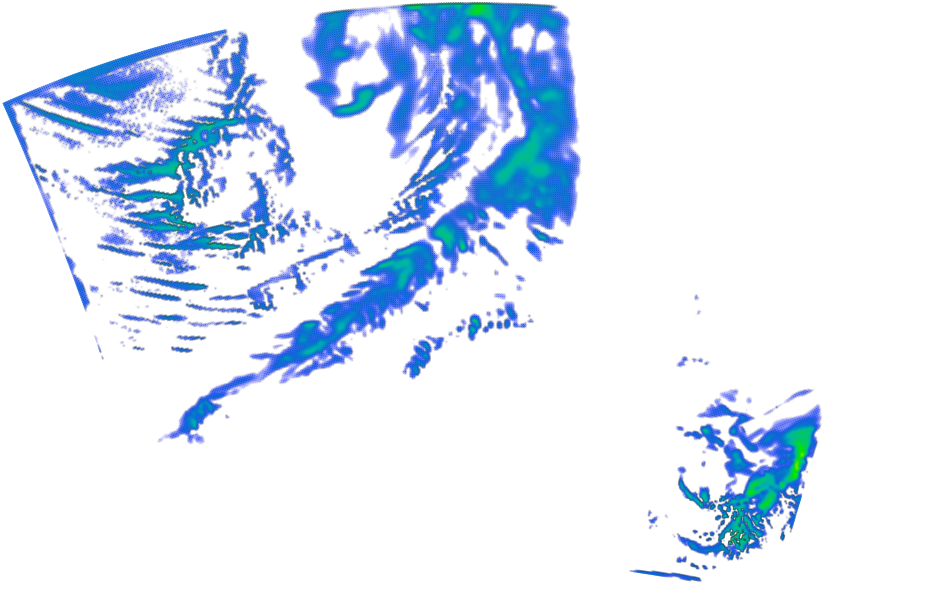
\includegraphics[scale=0.5]{Data/Mdrd_ukazka.png}
	\end{center}
	
	\subsection{Radar.bourky}
	
	Radar.bourky je datový zdroj který poskytuje data prostřednictvím snímků z radaru, data jsou tedy ve formátu bitmap. Tento datový zdroj je prakticky nepoužitelný pro určování budoucího počasí, protože poskytuje data pouze v aktuálním čase, mimo srážky neposkytuje jiné typy počasí a také pokrývá pouze Českou Republiku s blízkým okolím.
	
	Na druhou stranu tento zdroj uchovává informace o srážkách tři dny dozadu s časovým rozdílem pouhých 10 minut. Díky tomu se dá tento zdroj použít pro přesné zobrazení srážek v minulosti případně odhad počasí v následujících hodinách na základě velice přesného posunu hodnot na snímcích.
	
	Proto se zdroj využívá pouze pro určení srážek v aktuálním čase případně následujících šesti hodinách nebo pro určení srážek v minulých dnech s přesným posunem po deseti minutách.
	
	\subsection{Ukázka API a obsahu}
	
	Ukázka odkazu který vrací bitmapu obsahujících data o počasí Evropu v jednom aktuálním čase. Součástí ukázky je i samotná bitmapa \emph{Radar.bourky\_bitmapa} \cite{chmi}.
	
	http://radar.bourky.cz/data/pacz2gmaps.z\_max3d.20201001.1600.0.png
	
	\begin{center}
		\captionof{figure}{Snímek z radaru od Radar.bourky \cite{chmi}}
		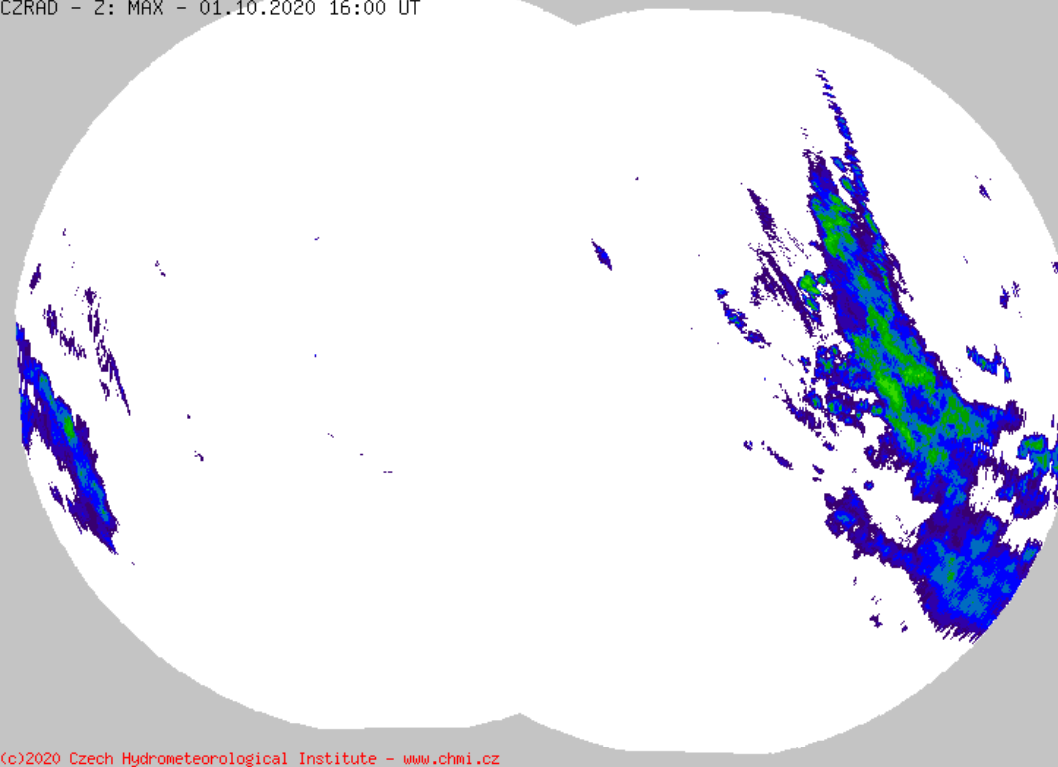
\includegraphics[scale=0.5]{Data/Rb_ukazka.png}
	\end{center}
	
	\section{Shrnutí použitých zdrojů}
	
	\begin{center}
		
		\captionof{table}{Shrnutí vlastností datových zdrojů}
		
		\begin{tabular} {l r c c c c c c c}
			
			Název & Typ dat & Počet dnů & Hodinový rozdíl & Stažení/min & Plocha & Typ \\
			\hline
			Yr.no & XML & 9 & 1 a 6 & & svět & s,v,t1,t2 \\ 
			OpenWeatherMap & JSON & 5 & 3 & 60 & svět & s,v,t1,t2 \\ 
			WeatherUnlocked & JSON & 5 & 3 & 75 & svět & s,v,t1,t2 \\ 
			Medard-online & BMP & 5 & 1 &  & Evropa & s,t1 \\ 
			Radar.bourky & BMP & -3 & 0.16 (10 min)& & ČR & s \\ 
			
			\multicolumn{7}{r}{\footnotesize *s = srážky, v = vlhkost, t1 = teplota, t2 = tlak}\\
			
		\end{tabular}
	\end{center}
	
	\chapter{Agregace dat}
	
	Při agregaci dat bylo zapotřebí vyřešit pár otázek. První z nich byla potřeba jednotného výstupního formátu pro různorodá vstupní data, tímto formátem byly zvoleny bitmapy obsahující data o jednom typu počasí, data jsou reprezentována pomocí barev a pokrávají určitou plochu pro určitý čas. Další otázkou bylo jak převádět barvy na číselné hodnoty a hodnoty zpět na barvy, tento problém vyřešilo využití škál. A nakonec jsme potřebovali pokrýt celou bitmapu pokud známe hodnotu počasí pro určité body, což nám vyřešila triangulace v kombinaci s interpolací.
	
	Každý z datových zdrojů je v agregaci dat realizován pomocí samostatné knihovny. Tato knihovna musí vždy implementovat rozhraní DataLoader a může využívat různé pomocné třídy pro správu dat o počasí jako je například triangulace nebo převod číselných hodnot na barvy a naopak. Dll soubor každé z knihoven je uložen do složky s datovými zdroji a následně je každá z knihoven datových zdrojů dynamicky načtena a zpracována pomocí reflexe třídou spravující agregaci dat.
	
	\section{Škála}
	
	Vzhledem k tomu že veškerá data o počasí jsou uložena do bitmap, ve který jsou data reprezentována barvou pixelů vzniká potřeba převádění barvy na číselnou hodnotu a naopak. Práce proto obsahuje metody, které pro určitou barvu vrátí desetinné číslo a pro určité číslo zase barvu.
	
	Nejprve tyto metody obsahovaly desítky podmínek které staticky kontrolovaly zda se jedná o konkrétní barvu, později zda barva patří do určitého rozmezí pro R, G, B složky. Tento přístup ale není vhodný, protože při potřebě změnit barvy pro určitá desetinná čísla vznikala nutnost přepsat hodnoty barev pro všechny metody ve veškerých podmínkách.
	
	Finálním řešením se stalo využití škál, škály jsou obrázky široké přesné tolik pixelů kolik hodnot uchovávají, kde každý pixel obsahuje unikátní barvu a reprezentuje jednu konkrétní číselnou hodnotu kterou daná barva reprezentuje. Výška škály může být pouze 1 pixel. Výhodou škál je, že změna barev reprezentujících hodnoty případně změna rozsahu uchovávaných hodnot se vyměnit pouze pomocí použití nové škály která bude opět orientovaná na šířku. Další z výhod je že metody které vrací hodnotu z barvy nemusí obsahovat desítky podmínek a stačí pouze vrátit hodnotu uloženou pro pixel. V programu jsou barvy ze škály uložený do slovníku, kde klíč reprezentuje barva a hodnotu desetinné číslo. Pro určení čísla z barvy stačí vypočítat index na kterém barva leží a tuto barvu vrátit.
	
	\section{Triangulace}
	
	Při vytváření bitmap dochází k určování hodnot počasí (teplota, srážky atp.) pro konkrétní zeměpisné souřadnice, které jsou následně převedeny na pixely bitmapy. Zjišťovat hodnotu pro každý jednotlivý pixel by bylo velice časově náročné, a protože můžeme předpokládat že v okolí pixelu budou obdobné hodnoty jako na pixelu samotné stačí nám určit hodnoty pouze pro určité množství pixelů rozložených správně po bitmapě. Následně je potřeba tyto pixely nějakým způsobem propojit, zde nám problém řeší využité triangulace.
	
	V práci se využívá S-hull Algoritmus pro triangulaci. Konkrétně Phil Atkinova implementace pro C\# \emph{S-hull} \cite{shull}. Algoritmus nám množinu bodů, v našem případě pixelů, rozdělí na trojúhelníky. Respektive nám pro každý vrchol řekne s kterými vrcholy je spojen hranou, čímž nám vznikne síť trojúhelníků pokrývající většinu bitmapy.
	
	%\vfill
	
	S-hull algoritmus slouží pro vytvoření Delaunayovi triangulace z množiny 2D bodů s časovou složitostí $O(n  log(n))$. Algoritmus využívá radiálního šíření, které se postupně vytváří z radiálně seřazené množiny 2D bodů, a je zakončen převracením trojúhelníků čímž se získá Delaunayova triangulace. Tento algoritmus ve srovnání s Q-hull algoritmem dosahuje přibližně polovičního času při vytváření triangulace pro náhodně generované množiny 2D bodů. S-hull je pro množinu unikátních 2D bodů $x_i$ implementován následovně:
	\begin{enumerate}
		\item Vybere počáteční bod $x_0$ z množiny bodů $x_i$.
		\item Seřadí body dle vzdálenosti od tohoto bodu $|x_i - x_0|^2$.
		\item Nalezne bod $x_j$, který je k bodu $x_0$ nejblíž.
		\item Nalezne bod $x_k$, který vytvoří nejmenší kružnici opsanou s body $x_0$ a $x_j$ současně i zaznamená střed kružnice opsané $C$.
		\item Seřadí body $x_0$, $x_j$, $x_k$ pro získání pravorukého systému, tohle je počáteční prvek pro convex hull.
		\item Přetřídí zbývající body na základě vzdálenosti bodů od středu kružnice opsané $|x_i - C|^2$ pro získání bodů $s_i$.
		\item Postupně se přidávají body $s_i$ do rostoucího 2D convex hull který je závislý na trojúhelníku vytvořeném z bodů $x_0$, $x_j$, $x_k$. Následné jsou přidány zkosené hrany pro 2D-hull, které jsou bodu viditelné z nově vytvořených trojúhelníků.
		\item Vzájemně se nepřekrývající triangulace pro množinu bodů je nyní vytvořena. Tato metoda je velice rychlá mezi způsoby vytváření 2D triangulace.
		\item Sousední páry trojúhelníků této triangulace musí být \uv{převráceny} aby došlo k vytvoření Delaunayovi triangulace z počáteční nepřekrývající se triangulace.
	\end{enumerate}
	
	\begin{center}
		\captionof{figure}{S-hull pro 500 náhodně generovaných bodů v matici 300x300}
		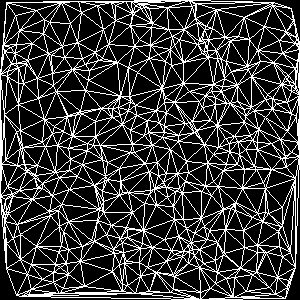
\includegraphics{Data/bmp_triangulace.png}
	\end{center}
	
	\section{Interpolace}
	
	Bitmapa je pokryta sítí trojúhelníků kde známe hodnotu každého vrcholu. Nyní vzniká potřeba každý trojúhelník vyplnit barvami, které reprezentují hodnotu pixelů uvnitř trojúhelníku. Tuto práci řeší využití interpolace, nebole výpočet hodnoty uvnitř objektu na základě vzdálenosti od vrcholů.
	
	Pro výpočet interpolace postačí jednoduchý vzorec \emph{Interpolace v trojúhelníku} \cite{interp}, který na základě hodnot vrcholů trojúhelníku a vzdálenosti od nich pro zjišťovaný bod určí jakou hodnotu sám zjišťovaný bod má.
	
	%\vspace{10mm}
	
	V prvním kroku výpočtu je zapotřebí spočítat vzdálenost $Distance$ zjišťovaného bodu $P$ od všech tří vrcholů trojúhelníku $V_1$, $V_2$, $V_3$ (\ref{eq_dist}). 
	
	\begin{equation}
		\begin{split}
			Distance_{v1} =\sqrt{(X_{v1}-P_x)^2+(Y_{v1}-P_y)^2} \\
			Distance_{v2} =\sqrt{(X_{v2}-P_x)^2+(Y_{v2}-P_y)^2} \\
			Distance_{v3} =\sqrt{(X_{v3}-P_x)^2+(Y_{v3}-P_y)^2}
		\end{split}\label{eq_dist}
	\end{equation}
	
	Následně se určí váha každého vrcholu $W$, neboli inverzní hodnota jeho vzdálenosti od zjišťovaného bodu (\ref{eq_w1}).
	
	\begin{align}\label{eq_w1}
		W_{v1} =\frac{1}{Distance_{v1}} &&
		W_{v2} =\frac{1}{Distance_{v1}} &&
		W_{v3} =\frac{1}{Distance_{v1}} 
	\end{align}
	
	Ve finální části výpočtu se určí hodnota našeho zjišťovaného bodu $Value_p$, která je úměrná podílu součtu součinů vah a hodnot jednotlivých vrcholů trojúhelníku se součtem jednotlivých vah (\ref{eq_val}).
	
	\begin{equation}\label{eq_val}
		Value_p = \frac{W_{v1}Value_{v1} + W_{v2}Value_{v2} + W_{v3}Value_{v3}}{W_{v1} + W_{v2} + W_{v3}}
	\end{equation}

	\section{Složky zdrojů}
	
	Každý z datových zdrojů má svou vlastní složku ze které čte a do které se ukládá informace.
	
	V této složce se nachází konfigurační JSON soubor obsahující informace na základě kterých si služba nastaví své parametry při vytvoření instance. Mezi tyto informace patří název datového zdroje včetně zkratky. Zeměpisné souřadnice zpracovávané plochy. Maximální dovolený počet stažení dat za minutu. Počet hodin který má služba zpracovávat zpětně, minimální potřebný hodinový rozdíl pro nové stažení dat a především poslední čas zpracování dat. Na základě posledního času zpracování bitmap a minimálního potřebného hodinového rozdílu datový zdroj určí zda dojde k vytváření nových bitmap či nikoli.
	
	Pokud zpracovává datový zdroj informace ve formě bitmap obsahuje tato složka i škálu daného datového zdroje. Pomocí této škály se převádí veškeré barvy na číselné hodnoty a následně za použití obecné škály služby zpět z čísla na normalizovanou barvu.
	
	Nejdůležitější soubory ukládané do složek jsou samotné bitmapy s daty o počasí. Bitmapy si do své složky každý zdroj ukládá při požadavku vytváření bitmap a následně je z této složky vrací při požadavku na poskytnutí dat o počasí pro daný typ a čas.
	
	\section{Zpracovávání dat}
	
	Při zpracování dat do bitmap záleží na tom jakým způsobem jsou data datovým zdrojem poskytována.
	
	Pokud jsou data poskytována ve formě bitmap potřebujeme zjistit jakou škálou jsou data v bitmapě zobrazena a rozsah zpracované plochy. Následně se musí bitmapa přeškálovat, teď jednotlivé pixely jsou převedeny na číselnou hodnotu pomocí škály služby a následně jsou čísla převedeny zpět na barvu za pomocí obecné škály pro agregaci dat využívané pro všechny zdroje na správu dat. Nakonec je potřeba správně pozicovat bitmapu, na základě zeměpisných souřadnic rohů bitmapy se zjistí jaká plocha je zpracována. Pokud je plocha příliš velká tak jak tomu je u zdroje Medard, dochází k vyřezání požadované části a následnému roztažení na 728x528 pixelů. Naopak u zdroje Yr.no je plocha příliš malá a tak dochází k patřičnému zmenšení bitmapy ze zdroje a napozicování do finální větší bitmapy.
	
	Data poskytována ve formátu XML či JSON se zpracovávají jiným způsobem. Nejprve měla každá služba svůj seznam měst nacházejících se ve zpracovávané ploše pro který poskytuje informace o počasí. Pro každé z těchto měst se určilo počasí a 
	pozice pixelu reprezentujícího dané město. Pixel se následně vykreslil na mapu a pomocí triangulace se vytvořilo síť trojúhelníků, které se ve finále vybarvily. Tento způsob nebyl vhodný protože nepokrýval celou bitmapu rovnoměrně, v určitých místech chyběly informace a naopak v jiným místech bylo příliš mnoho bodů u sebe, proto se způsob zpracování změnil.
	
	Aktuálně dochází k cyklickému průchodu bitmapou s posunem 25 pixelů na výšku a šířku. Každý z těchto pixelů je převeden na zeměpisné souřadnice na základě vzdálenosti od levého horního rohu přičemž dochází k určení počasí v tomto bodě. Počasí je následně uloženo do slovníku kde klíč tvoří čas dané předpovědi a hodnotou je list počasí pro stejný čas v různých bodech. Nakonec je pro každý z časů proveden průchod listem, vykreslení pixelů na své pozice, následuje vytvoření sítě trojúhelníků pomocí triangulace zakončená s vybarvením jednotlivých trojúhelníků využitím interpolace. Pro každý čas je vytvořeno tolik bitmap kolik parametrů počasí daná služba zpracovává. Počet jednotlivých časů je úměrný počtu všech dostupných předpovědí pro všechny body.
	
	Použití triangulace není při zpracovávání rovnoměrně vzdálených bodů nutné, každopádně se v práci pro zpracování dat ponechala. Datové zdroje takto mohou zpracovávat i nerovnoměrně vzdálené body a pokud by došlo ke změně implementace určení dat v daných bodech, tedy pro jednotlivé časy by se body neurčovali cyklicky ale opět pomocí seznamu různě umístěných měst ve zpracované ploše, triangulace by se postarala o rozdělení bodů na síť trojúhelníků s následným vybarvením pomocí interpolace.
	
	\begin{center}
		\captionof{figure}{Body reprezentující teplotu na ploše}
		
\includegraphics[scale=0.5]{Data/bmp_body.png}
	\end{center}
	
	\begin{center}
		\captionof{figure}{Síť trojúhelníků pro bitmapu teploty}
		
\includegraphics[scale=0.5]{Data/bmp_sit.png}
	\end{center}
	
	\begin{center}
		\captionof{figure}{Kompletní bitmapa pro teplotu}
		
\includegraphics[scale=0.5]{Data/bmp_vybarvena.png}
	\end{center}
	
	\section{Ukládání dat}
	
	Veškerá zpracovaná data je potřeba uložit aby bylo možné je posléze poskytovat a nemuseli se pravidelně při každém dotazu o data generovat znovu. Vzhledem k tomu že se ukládají data o počasí na ploše nemá smysl používat žádnou databázi protože by bylo zbytečně složité ukládat celou předpověď pro každý bod zvlášť i když by bod vedle obsahovat obdobné, ne-li úplně totožné údaje. Právě proto se zvolilo ukládání dat do bitmap které nám jednoduše pokryjí celou zpracovanou plochu.
	
	Výhodou bitmap je že pro jeden zvolený čas dokáží pokrýt velkou plochu a tím pádem stačí jeden soubor pro určitý čas. Nevýhodou je, že bitmapa nám poskytuje data pouze o jedné hodnotě počasí, například o teplotě, a proto pokud požadujeme zjišťovat více vlastností počasí v jedno chvíli musíme pro každý typ uložit jednu samostatnou bitmapu s těmito daty.
	
	Jednotlivé datové zdroje ukládají své bitmapy se jménem $TYP-ČAS$ a na základě tohoto jména je následně možné bitmapy vracet. Prefix názvu matice pojmenovaný jako $TYP$ reprezentuje typ předpovědi která bitmapa zpracovává, pro teplotu to je $TEMP$, srážky $PREC$ a tak podobně. Druhé části názvu zvané $ČAS$ je uložený čas pro většinu datových zdrojů ve formátu $ROK-MĚSÍC-DEN-HODINA$. Vzhledem k tomu že datové zdroje poskytují předpovědi pro časy vzdálené v řádu hodin je zbytečné ukládat do názvu času minuty nebo sekundy. Pouze jediný z datových zdrojů Radar.bourky poskytuje data o počasí v rámci minut s posunem po 10 a proto je pro tento zdroj zahrnut i parametr minut v časové části názvu $ROK-MĚSÍC-DEN-MINUTA$.
	
	To pro jakou plochu datové zdroje zpracovávají své bitmapy je dopředu určeno a proto nemá smysl tento údaj ukládat přímo do bitmap.
	
	Každý z datových zdrojů ukládá do své složky zpracované bitmapy a následně při určitých dotazech tyto bitmapy vrací. 
	
	\section{Poskytování dat}
	
	Datové zdroje po obdržení informací o typu počasí a času dokáží vrátit správnou bitmapu, která je vybrána dle svého názvu. Název typu počasí se musí shodovat s prefixem názvu bitmapy $typ$. Požadovaný čas předpovědi si každý z datových zdrojů umí správně zaokrouhlit aby bylo jasné jaká bitmapa tento čas zpracovává. Pokud datový zdroj poskytuje data každých 10 minut je čas zaokrouhlen na desítky minut dolů. Při poskytování dat každou hodinu je k času přičteno 30 minut a následně je tento čas zaokrouhlen na hodiny dolů. Poslední možností je vracení času jednou za 3 nebo 6 hodin, v tomto případě se zjistí ke které časové hranici má zadaný čas blíže a tato varianta je zvolena.
	
	Zaokrouhlený čas je následně převeden do formátu $ROK-MĚSÍC-DEN$, případně včetně $MINUTA$ pro Radar.bourky. V tuto chvíli zná datový zdroj celý název hledané bitmapy a tu jednoduše vrátí. Pokud bitmapa neexistuje dojde k vyvolání výjimky.
	
	Pokud datový zdroj vytváří bitmapy nekonzistentně, například prvních pár dnů je s rozestupem 1 hodiny a zbytek s rozestupem 6 hodin tak jak to dělá například Yr.no, dochází při nenalezení bitmapy se zaokrouhleným časem k sekvenčnímu průchodu všech zpracovaných bitmap a vrácení bitmapy s nejbližším časem k požadovanému času. Tato bitmapa je vrácena pouze tehdy pokud je odchylka času maximálně 6 hodin v opačném případě dochází opět k vyvolání výjimky.
	
	\chapter{Distribuce dat}
	
	Shromážděné a zprůměrované předpovědi počasí je potřeba nějakým způsobem dodávat klientovi. Tuto úlohu nám splní webová služba, která pro různé dotazy ve formě url API vrací agregovaná data o počasí v požadovaných formátech. Služba se implementovala jako MVC aplikace pro C\# a využívá pro svou práci knihovnu pro agregaci dat z předešlé sekce. Vzhledem k tomu že jsou data o počasí uložená do bitmap, lze informace o počasí poskytovat i bez připojení k internetu, musíme však mít pro dané časy bitmapy dopředu vytvořené. Služba volá požadavek o vytvoření bitmap vždy při spuštění a následně každou další hodnu běhu, jednotlivé datové zdroje si následně zjistí kdy byly bitmapy naposledy vytvořený a pokud již uplynul minimální čas dojde k vytváření bitmap nových, tento čas se může u každého datového zdroje lišit.
	
	\section{API}
	
	Při práci se službou se využívá vytvořeného API které pro správně zadané vstupní parametry vrací požadovanou předpověď. Webová služba vrací data ve třech formátech XML, JSON a bitmapa. Nakonec je možné získat jednotlivé škály, které služba využívá pro správu dat o počasí v bitmapách.
	
	\subsection{Bitmap předpověď}
	
	Tato předpověď se získává požadavkem bmp a vždy vrací bitmapu o rozměrech 728x528 pixelů pokrývající určitou plochu. Plocha je vymezená body zeměpisných souřadnic, konkrétně levým horním $p1$ a pravým dolním $p2$ rohem. Pokud nedojde k zadání těchto bodů je bitmapa určena pro Českou republiku. Při určování této předpovědi je zapotřebí rovněž i čas pro který se má předpověď určitě $time$, tento čas musí být ve formátu ISO 8601 a pokud není zadán nebo je místo něj vyplněna hodnota 0 určí se předpověď pro aktuální čas požadavku předpovědi. Následně je potře zadat typ předpovědi $type$, který má bitmapa reprezentovat tyto typy jsou 2 typ prec reprezentuje srážky v mm a typ temp teplotu ve stupních Celsia. Nakonec se zadávají datové zdroje $loaders$, takzvané loadery, ze kterých má služba získávat data. Je potřeba zadat zkratky loaderů oddělené čárkami pro každý loader který má služba využít pokud není zadán žádný loader použijí se všechny dostupné současně.
	\\\\
	adresaserveru/bmp?type=\{typ\}\&time=\{čas\}\&loaders=\{datové zdroje\}\&p1=\{bod1\}\&p2=\{bod2\}
	
	\begin{center}
		
		\captionof{table}{Parametry bitmap předpovědí}
		
		\begin{tabular}{c c p{13cm}}
			Název & Povinnost & Význam \\
			\midrule
			type & ANO & Typ předpovědi, určuje druh vykreslených informací. Například typ $prec$ reprezentuje srážky v milimetrech a typ $temp$ teplotu ve stupních Celsia.\\ 
			time & NE & Čas předpovědi, pokud je zadán musí být ve formátu ISO 8601. Pokud zadán není nebo je zadána hodnota 0  provede se předpověď pro aktuální čas.\\ 
			loaders & NE & Datové zdroje které se mají použít. Výběr datových zdroju se provede zadáním zkratek jednotlivých zdrojů oddělených čárkami. Pokud je parametr prázdný použijí se veškeré datové zdroje služby. \\ 
			p1 & NE & Levý horní roh vymezující plochu bitmapy. Bod reprezentuje zeměpisné údaje v pořadí zeměpisná šířka a délka (latitude a longitude), údaje jsou odděleny čárkou. Pro oddělení celé a desetinné části souřadnice se používá tečka. Pokud bod $p1$ a $p1$ není zadán, bitmapa se vykreslí pro celou možnou plochu.\\
			p2 & NE & Pravý dolní roh vymezující plochu bitmapy. Bod reprezentuje zeměpisné údaje v pořadí zeměpisná šířka a délka (latitude a longitude), údaje jsou odděleny čárkou. Pro oddělení celé a desetinné části souřadnice se používá tečka. Pokud bod $p1$ a $p1$ není zadán, bitmapa se vykreslí pro celou možnou plochu.\\
		\end{tabular}
	\end{center}
	
	Příklady požadavků:
	\begin{itemize}
		\item Požadujeme bitmapu s daty o teplotě pro aktuální čas, která pokrývající celou možnou plochu a využívá veškeré datové zdroje.
		\begin{itemize}
			\item adresaserveru/bmp?type=temp
		\end{itemize}
		\item Požadujeme bitmapu s daty o srážkách pro 26. 5. 2021 18:30, která pokrývající celou možnou plochu a využívá datové zdroje od služeb OpenWeatherMap a Yr.No.
		\begin{itemize}
			\item adresaserveru/bmp?type=prec\&time=2021-05-26T18:30:00\&loaders=owm,yrno
		\end{itemize}
		\item Požadujeme bitmapu s daty o srážkách pro aktuální čas, která pokrývající město Olomouc a využívá datový zdroj od služby Medard-Online.
		\begin{itemize}
			\item adresaserveru/bmp?type=prec\&p1=49.621559,17.1507294\&p2=49.5211889,17.4213141\&loaders=mdrd
		\end{itemize}
	\end{itemize}
	
	\subsection{XML a JSON předpověď}
	
	Tento požadavek nám dovoluje získat data o počasí pro určitý bod v zadaném čase, případně lze určit data o počasí pro více časů za sebou s konstantním hodinovým rozdílem. Při získávání XML nebo JSON dat potřebujeme zadat stejně jako u bitmap předpovědí zadat parametr požadovaného času $time$ a datové zdroje které tento čas zpracovávají $loaders$. Dále musíme zadat požadovaný typ dat XML/JSON $data$ a zeměpisný bod pro který chceme počasí určit, bod se skládá z parametrů $lon$ a $lat$. Pro získání více časových oken v jedné předpovědi musíme přidat parametr reprezentující počet předpovědí $numOfFcs$ a hodinový rozdíl mezi těmito předpověďmi $hourDif$.
	\\\\
	adresaserveru/{data}?time={čas}\&lat={zeměpisná\_šířka}\&lon={zeměpisní\_délka}\&loaders={datové\_zdroje}
	
	adresaserveru/{data}?time={čas}\&numOfFcs={počet\_předpovědí}\&hourDif={hodinový\_rozdíl\_mezi\_předpověďmi}\&lat={zeměpisná\_šířka}\&lon={zeměpisní\_délka}\&loaders={datové\_zdroje}
	
	\begin{center}
		
		\captionof{table}{Parametry XML/JSON předpovědí}
		
		\begin{tabular}{c c p{13cm}}
			Název & Povinnost & Význam \\
			\midrule
			data & ANO & Formát v jakém mají být data o počasí zpracována. Rozlišujeme dva typy a to $xml$ a $json$.\\
			lon & ANO & Longitude, parametr reprezentující zeměpisnou délku požadované souřadnice. Desetinná a celá část souřadnice jsou odděleny tečkou.\\
			lat & ANO & Latitude, parametr reprezentující zeměpisnou šířku požadované souřadnice. Desetinná a celá část souřadnice jsou odděleny tečkou.\\
			time & NE & Čas předpovědi, pokud je zadán musí být ve formátu ISO 8601. Pokud zadán není nebo je zadána hodnota 0  provede se předpověď pro aktuální čas.\\ 
			loaders & NE & Datové zdroje které se mají použít. Výběr datových zdrojů se provede zadáním zkratek jednotlivých zdrojů oddělených čárkami. Pokud je parametr prázdný použijí se veškeré datové zdroje služby. \\
			numOfFcs & NE & Počet časových oken které má předpověď obsahovat. Pokud není tento parametr zadán, v předpovědi bude právě jedno časové okno pro zadaný čas.\\
			hourDif & NE & Hodinový rozdíl mezi jednotlivými časovými okny v předpovědi. Pokud není tento parametr zadán, v předpovědi bude právě jedno časové okno pro zadaný čas.\\
		\end{tabular}
	\end{center}
	
	Příklady požadavků:
	\begin{itemize}
		\item Požadujeme předpověď o počasí pro aktuální čas v Ostravě zpracovanou všemi datovými zdroji ve formátu XML.
		\begin{itemize}
			\item adresaserveru/xml?lon=18.262524\&lat=49.820923
		\end{itemize}	
		\item Požadujeme předpověď o počasí pro datum a čas 14.03.2021 18:35 v Ostravě zpracovanou všemi datovými zdroji ve formátu JSON.
		\begin{itemize}
			\item adresaserveru/json?lon=18.262524\&lat=49.820923\&time=2021-03-14T18:35:00
		\end{itemize}
		\item Požadujeme předpověď o počasí pro datum a čas 14.03.2021 18:35 v Ostravě zpracovanou datovými zdroji OpenWeatherMap a WeatherUnlocked ve formátu XML.
		\begin{itemize}
			\item adresaserveru/xml?lon=18.262524\&lat=49.820923\&time=2021-03-14T18:35:00\&loaders=owm,weun
		\end{itemize}
		\item Požadujeme předpověď o počasí v Ostravě pro 5 časových oken s 3 hodinovými rozestupy počínaje aktuálním časem.
		\begin{itemize}
			\item adresaserveru/json?lon=18.262524\&lat=49.820923\&time=2021-03-14T18:35:00\&numOfFcs=5\&hourDif=3
		\end{itemize}
	\end{itemize}
	
	\subsection{Využívané škály}
	
	Při stahování bitmap obsahujících data o počasí je vhodné mít prostředek na převod barev z jednotlivých pixelů na číselné hodnoty. Právě pro tento účel slouží škály.
	
	Služba nám proto umožňuje stažení jednotlivých škál, které používá při zpracovávání bitmap s daty o počasí. Stačí znát zkratku typu počasí a služba nám vrátí využívanou škálu.
	
	Příklady požadavků:
	\begin{itemize}
		\item Požadujeme škálu pro teploty.
		\begin{itemize}
			\item adresaserveru/scale?type=temp
		\end{itemize}
		\item Požadujeme škálu pro srážky.
		\begin{itemize}
			\item adresaserveru/scale?type=prec
		\end{itemize}
	\end{itemize}
	
	\subsection{Zkratky typů počasí}
	
	Zkratky pro jednotlivé typy předpovědí které se využívají v parametru type.
	
	\begin{center}
		
		\captionof{table}{Zkratky typů předpovědí}
		
		\begin{tabular}{c c c}
			Typ počasí & Jednotka & Zkratka pro API\\
			\midrule
			Srážky & mm & prec \\
			Teplota & °C & temp \\
			Tlak & hPa & pres \\
			Vlhkost & \% & humi \\
		\end{tabular}
	\end{center}
	
	\subsection{Zkratky datových zdrojů}
	
	Zkratky pro jednotlivé datové zdroje které se využívají v parametru loaders. Při použití více zkratek za sebou oddělených čárkou dojde k použití více zdrojů současně.
	
	\begin{center}
		
		\captionof{table}{Zkratky datových zdrojů}
		
		\begin{tabular}{c c}
			Celý název datového zdroje & Zkratka pro API\\
			\midrule
			Radar.bourky & rb \\
			Medard-online & mdrd \\
			OpenWeatherMap & owm \\
			Yr.no & yrno \\
			WeatherUnlocked & weun \\
		\end{tabular}
	\end{center}
	
	\section{Chyba při zpracování dat}
	
	Při požadavku o dodání dat může dojít k chybě, nejčastěji při chybném zadání parametrů v API, případně i při požadování dat pro čas který ještě bitmapami není zpracován. Pokud tato situace nastane služba místo požadovaných dat vrátí text ve formátu JSON obsahující jediný parametr $message$ obsahující informace proč k pádu došlo a jak parametry upravit aby se chyba neopakovala a bylo možné nějaké informace o počasí získat.
	
	\chapter{Vizualizace dat}
	
	Část vizualizace dat je realizována prostřednictvím desktopové aplikace Bude-hezky napsané v C\# Windows Forms. Aplikace umožňuje uživateli zobrazit informace o různých typech počasí v bodě či na trase pro zvolený čas. Předpověď je zároveň tvořena grafem a bitmapou barev pokrývající zobrazenou plochu. Data jsou distribuována webovou službou a uživatel si může zvolit které datové zdroje chce pro své předpovědi používat.
	
	\section{Obecné použití}
	
	Aplikace je tvořena několika vzájemně propojenými částmi mapou reprezentující plochu pro kterou chceme znát počasí, lištou času pro který nebo od kterého chceme počasí určit, radio buttony reprezentující typ předpovědi, comboboxy pro volbu datových zdrojů, grafem zobrazující počasí pro více časových intervalů, tlačítkem pro přehrání animace počasí společně s nastavitelnými parametry této animace a nakonec meníčkem pro nastavení aplikace případně volby určitých akcí.
	
	Při používání aplikace si uživatel zvolí který typ počasí chce zobrazit vybráním patřičného radio buttonu a které z datových zdrojů si přeje používat zakliknutím požadovaných check boxů. Následně je potřeba zvolit čas první předpovědi reprezentovaný spodní lištou. Při každé změně času, typu počasí nebo datového zdroje dojde k vykreslení bitmapy na mapu. Bitmapa reprezentuje počasí na ploše a při změně pozice na mapě nebo změně přiblížení se bitmapa patřičně překreslí.
	
	Typy počasí odpovídají veškerým typům poskytovaným webovou službou, jedná se tedy o srážkám, teplotu, tlak a vlhkost. Pro datové zdroje se rovněž používají veškeré datové zdroje které služba poskytuje. Lišta dat a časů 
	je pokryta časy od šesti hodin zpět po 5 dnů dopředu od aktuálního času a krokuje se po deseti minutách.
	
	Při určování číselných hodnot z bitmap se využívají totožné škály které webová služba používá při vyvážení samotných bitmap. Tyto škály si vizualizační aplikace dokáže stáhnout a přepsat pokud dojde k jejich změně na straně webové služby.
	
	\section{Mapa}
	
	Pro vykreslení a práci s mapou se nejprve používala komponenta MapWinGIS která poskytovala veškeré potřebné vlastnosti, naneštěstí bylo zapotřebí tuto komponentu nejdříve na zařízení nainstalovat a až poté ji mohla aplikace využívat. Tento důvod způsobil nutnost výměny komponenty za konkurence schopnou alternativu.
	
	Pro práci s mapou se nakonec využívá komponenta GMap.NET, která je volně dostupná pro rozšíření vlastností Windows Forms. Tato komponenta nám umožňuje vykreslit mapu po které se může uživatel pohybovat, přibližovat a oddalovat ji. Komponenta dokáže určit zeměpisné souřadnice bodu ve kterém se nachází kurzor myši, takže není problém určit souřadnice požadovaného místa a ani plochy pro kterou data určujeme protože ta je vyhrazena levým horním a pravým dolním rohem mapy. Komponenta nám dovoluje přidat značky s popisky na mapu pokud máme za potřebí vyznačit zjišťovaný bod či body na trase, pro trasu se krom bodů vykreslí i křivka reprezentující celou cestu. Do mapy máme také možnost přidat bitmapu což se využívá při nakreslení dat.
	
	Na samotné mapě se vždy při změnách času, typu a zdrojů vykresluje bitmapa reprezentující počasí, průhlednost této bitmapy má uživatel možnost nastavit prostřednictvím nastavení v menu.
	
	\section{Počasí v bodě}
	
	Při určování počasí v bodě stačí dvakrát kliknout do mapy na místo kde chceme zjistit přesnou hodnotu počasí. Následně se na tomto bodě vykreslí značka s popiskem reprezentujícím hodnotu počasí v tomto bodě. Při opětovném kliknutí na značku dojde k jejímu odstranění. Součástí předpovědi je i zobrazení grafu pod mapou, graf reprezentuje počasí v zvoleném bodě od počátečního času, teda času nastaveném na liště a každý další sloupec grafu zobrazuje počasí pro stejný bod v čase inkrementovaném o hodinu. Počet sloupců je nastavitelný.
	
	Při zjišťování počasí v bodě se využívají data z bitmapy kterou si aplikace stáhla z webového serveru ve chvíli co byl zvolen typ počasí, datový zdroj a čas. Z této bitmapy se určí pixel obsahující data o počasí pro požadovaný bod a pomocí škály je RGB hodnota převedena na desetinné číslo.
	
	\section{Počasí na trase}
	
	Mimo počasí pro jeden bod v různých časem máme možnost vykreslit i počasí na určité trase, tedy na více různých bodech v rozdílných časech na základě rychlosti pohybu. Trasa se zadává pomocí předem vytvořeného GPX souboru obsahujícího body reprezentující samotnou trasu. Při zobrazování trasy je potřeba zjistit jakou rychlostí se po trase postupuje pro možnost zjištění postupu času na následující bodech zvolené cesty. Tato rychlost se v aplikaci může určit dvěma způsoby. Prvním je zadání počátečního času a dopravního prostředku, každý dopravní prostředek má svou vlastní předem nastavenou rychlost a při výpočtu uplynulé vzdálenosti od počátku dokážeme určit i čas v tomto uplynulém bodě. Druhým způsobem určení času na trase je zadání času začátku cesty a času konce cesty, díky těmto informacím dokážeme určit jak dlouho trvá urazit celou cestu a tím pádem dokážeme spočítat i rychlost, když známe délku cesty.
	
	Při požadavku o zobrazení počasí v trase musí uživatel vybrat možnost $Akce$ z menu a v něm zakliknout $Nahrát trasu z GPX souboru$. Poté si uživatel vybere jednu z možností určení rychlosti dopravy, zadá tedy počáteční čas a dopravní prostředek případně počáteční a koncový čas. Nakonec vybere cestu k samotnému GPX souboru. Pokud během toho procesu dojde k jakékoliv chybě proces se ukončí a uživateli se vypíše co přesně neproběhlo správně.
	
	Po úspěšném zadání všech parametrů a zpracování souboru je na mapě nakreslena křivka reprezentující trasu. Na této křivce je zobrazeno 10 bodů oddělených rovnoměrně od sebe, každý bod obsahuje popis informací o počasí v tomto bodě. Součástí zobrazení trasy je i vykreslení grafu pod mapou, graf obsahuje 10 sloupců kde každý sloupec reprezentuje jeden z vyznačených bodů na trase. 
	
	Určování dat pro počasí v těchto bodech se provádí stejně jako v určování informací o počasí v bodě. Pro každý vykreslený bod na trase s rozdílným časem se stáhne nová bitmapa na které se najde pixel reprezentující danou zeměpisnou souřadnici a pro tento pixel se určí hodnota počasí převodem RGB hodnoty na desetinné číslo prostřednictvím škály.
	
	\section{Animace počasí}
	
	Uživatel má možnost zobrazit si animaci předpovědí pro zvolený typ počasí od zvoleného počátečního času. Při kliknutí na tlačítko pro přehrání animace dochází k vykreslení bitmap předpovědí pro zvolený typ počasí, čas počasí pro animaci začíná od zvoleného času na liště, následně se v animaci vykreslují nové bitmapy pro následující čas inkrementovaný o zvolený interval. Intervaly se pohybují v hodnotách 10min, 30min, 1h, 3h a 6h. Počet kroků animace je rovněž nastavitelný a dodává nám možnost zobrazit průběh počasí pro dlouhé či krátké úseky času. Při běhu animace můžeme vidět v jakém časovém úseku se právě nacházíme a kolikátý snímek z celkového počtu je aktuálně zpracováván.
	
	Při zpracování animace dochází k cyklickému stahování bitmap z webové služby. Hranice bitmapy jsou ohraničeny souřadnicemi rohů mapy a čas této předpovědi je vždy o hodinu vyšší než měla předpověď předešlá. Typ počasí ani datové zdroje se u animace neliší ty jsou pro celou animaci stejné.
	
	\section{Graf}
	
	Součástí aplikace je i graf obsahující informace o předpovědích pro jednotlivé časy. Šířka grafu se dynamicky mění při změně rozměrů okna aplikace. Graf má na ose $y$ sloupce ukazující hodnotu daného typu počasí v rozmezí od minima do maxima, na ose $x$ se nachází čas předpovědi pro daný sloupce. Graf je vykreslován na panel pomocí základních metod knihovny System.Drawing, nevyužívají pro tento účel se žádné externí knihovny. Barva sloupců společně s jejich počtem v grafu je nastavitelná.
	
	Při vykreslování grafu pro bod reprezentují všechny sloupce stejné místo s rozdílným časem. Časy jsou od sebe posunuté o hodinu a počet vykreslených sloupců lze změnit v nastavení.
	
	Pro tuto předpověď nám graf vykresluje počasí pro 8 rovnoměrně vzdálených míst na trase. Proto počet sloupců v tomto grafu je vždy 8. Na rozdíl od grafu pro předpověď v bodě nám tento graf na ose $x$ reprezentuje čas sloupce v aktuálním bodě a vzdálenost tohoto bodu od počátku cesty.
	
	Zobrazený typ jednotek předpovědi na ose $y$ se mění dle zvoleného typu počasí v radio buttonech. Každý typ předpovědi zdá své jednotky a mimo to i minimální a maximální hodnotu počasí pro tuto jednotku. Hodnota předpovědi pro každý sloupec se tedy určí jako procentuální hodnota v rozmezí od minima po maximum.
	
	Pokud graf aktuálně nevykresluje žádné informace tak je v poli určeném pro sloupce vypsán text popisující co pole reprezentuje a kdy zde dojde k vykreslení dat. Nejprve bylo pole úplně prázdné a neobsahovalo žádný text čímž v aplikaci vznikla velká bílá plocha bez účelu, takto uživatel na první pohled ví k čemu tam tato plocha je. Tento text v poli je vždy vypsán při startu aplikace a následně spuštění animace nebo při vymazání zobrazené předpovědi.
	
	\section{Nastavení a akce}
	
	Součástí aplikace je i menu nacházející se v horní liště. Menu je rozděleno do části nastavení pro individuální změny aplikace a akce pro rychlé volby.
	
	V části nastavení lze nastavit adresu webové služby poskytující data o počasí. Dále se zde nachází možnost změny průhlednosti vykreslené bitmapy na samotnou mapu, lze vybrat vlastní hodnotu v rozmezí od 0 do 255 kde 0 je naprosto průhledná bitmapa a 255 bitmapa bez jakékoliv průhlednosti je zde i volba pro přímé nastavení minima či maxima bez potřeby zapisovat hodnotu ručně. Následně zde lze nastavit počet vykreslených sloupců v grafu při určování počasí v bodě. Všechny tyto hodnoty se musí nacházet v předem definovaném rozmezí od minima po maximum, při zadání neplatné hodnoty dojde k nastavení nejbližší platné. Nastavení obsahuje i možnost změny barvy sloupců grafu a nakonec zde lze i stáhnout nové škály z webové služby pro určování číselných hodnot z RGB pixelů. Při potřeba nastavení výchozích hodnot lze v nastavení zvolit i tuto variantu.
	
	Součástí tohoto nastavení byla i možnost změny počtu kroků při animaci a změna časového intervalu mezi jednotlivými kroky. Změny těchto parametrů se nakonec přesunuly přímo do aplikace vedle tlačítka pro spuštění animace. K této změně došlo protože se předpokládá že tyto parametry se budou pravidelně měnit a proto je zbytečné je mít schované v sekci s nastavením prvků které se změní pouze jednou případně velice výjimečně.
	
	V části menu akce je na výběr mezi vybráním cesty z GPX souboru pro vykreslení trasy a určení počasí na ni. Druhá možnost v akcích je přemazání mapy. Tato volba slouží k vymazání hodnot na mapě. Při této volbě dojde k smazání grafu, bitmapy počasí na mapě a značce označující počasí v bodě případně se odstraní trasa společně s jejími body a popisy.
	
	Veškeré nastavení aplikace se ukládá do konfiguračního JSON souboru. Při spuštění aplikace se z tohoto souboru načtou data o adrese serveru, průhlednosti bitmapy, počtu kroků při animaci, počtu předpovědí pro počasí v bodě, poslední zvolený typ počasí a naposledy zvolené datové zdroje. Díky tomuto souboru nemusí uživatel při každém spuštění znovu nastavovat veškeré věci znovu. Při změně jakéhokoliv z těchto atributů dochází k přepsání JSON souboru pro udržení neustále konzistence s aplikací po ukončení aplikace a opětovném spuštění.
	
	\section{Chyby při zobrazování dat}
	
	Pokud dojde k chybě při získávání dat ze serveru vypíše se chybová hláška vrácená samotnou službou jako atribut message v chybovém JSON výstupu. K těmto chybám dochází nejčastěji při pokusu o získání počasí pro čas pro který nemá žádný ze zvolených datových zdrojů vytvořenou bitmapu. Pokud dochází k pádu z neznámého důvodu dochází k výpisu obecné chyby a prosba o kontrolu zda je webová služba aktuálně dostupná.
	
	Může se stát že dojde k chybě i při určování počasí trasy z GPX soboru. Mimo pád při neschopnosti zjištění počasí pro daný bod dochází i k chybě při zpracování samotného GPX soboru při nepodporovaném formátování. Případně dochází k chybě při zadání většího počátečního času než toho koncového. Při těchto chybách dochází k oznámení informaci uživateli proč došlo k chybě a možnost napravení chyb při novém vykreslení trasy.
	
	\chapter{Závěr}
	
	\printbibliography[title={Literatura}, heading=bibintoc]
	
	
\end{document}
